\documentclass{article}

\usepackage{fullpage}
\usepackage{amsmath}
\usepackage{amssymb}
\usepackage{graphicx} 
% \marginparwidth = 35pt
\usepackage[norsk]{babel}              % norske navn rundt omkring
\usepackage[T1]{fontenc}              % gir tilgang til alle tegn i fonten
\usepackage[utf8]{inputenc}         % utf8 rules them ALL
\usepackage{parskip}
\usepackage{multirow}
\usepackage{listings}
\usepackage[table]{xcolor}
\usepackage{fancyhdr}
\usepackage{hyperref}

% forside 
\newcommand{\PageTitle}{Detaljert Brukermanual}
\newcommand{\DateDeadline}{\today}

% SAKSMACRO
\newcommand{\sak}[2]{\section*{Sak #1: #2}}

% Bildemakro 
\def\imagetop#1{\vtop{\null\hbox{#1}}}



\begin{document}
% Importert fra fil 
\newcommand{\HRule}{\rule{\linewidth}{0.5mm}}
\begin{titlepage}
	\vspace*{3cm}
	\begin{center}
		{\Large RMI med prosjekt i distribuerte systemer TDAT3014}
		\HRule \\[0.5cm]
		{\LARGE\textsc{\textbf{\PageTitle}}}
		\HRule \\[1.0cm]
		{\large \DateDeadline} 
		\vspace{\fill}
		\begin{flushleft}
		\emph{Gruppemedlemmer}:\\
			{Andreas Mosti, \ Thomas Mowatt} 
		\end{flushleft}
	\end{center}
\end{titlepage}



\newpage
.\vfill
\begin{centering}
\LARGE


\textit{Et dokument om}  \\ 
\ \textit {Simple Network Server -} \\ 
\ \textit {Produktet}
\vspace{12cm}
\hspace{15cm}
\newpage
\end{centering} 
\fancyhead[L]{
Simple Network Server		\hfill			 Version: 1.0 \\
Detaljert Brukermanual 	\hfill			Date: \today  \\}
\pagestyle{fancy}
\setlength\headsep{30pt}


\begin{table}[h] % http://en.wikibooks.org/wiki/LaTeX/Tables

\caption{Revisjonshistorikk}
	\begin{tabular}{| m{3cm} | m{1cm} | m{5cm} | m{4cm} |} 
	\hline	
	Dato & Versjon & Beskrivelse & Forfatter\\ 
	\hline
	 02/02/13> & 1.0 & Established requirements document & Andreas Mosti og Thomas Mowatt\\ 
	\hline
	<25/02/13> & 1.1 & Edited document according to the feedback & Andreas Mosti og Thomas Mowatt\\ 
	\hline
	<28/04/13> & 1.2 & Final version & Andreas Mosti og Thomas Mowatt\\ 
	\hline
	
	\end{tabular}
\end{table}

\newpage

\tableofcontents
\newpage
\section{Introduksjon}
\subsection{Mål}
Dette dokumentet er ment som brukermanual for Simple Network Server - produktet. Det vil inneholde alt som trengs for å kunne bruke løsningen fullt ut, inkludert avhengigheter og oppsett.
\subsection{Omfang}
Dette dokumentet omhandler bruk av hele systemet. \\ Beskrevet miljø er Linux (Debian - basert) og Mac OS X 10.9.
\\ MERK: Prosjektet er tilgjengelig for Windows, men dette er ikke testet. 
\subsection{Definisjoner, akronymer, forkortelser}
\begin{itemize}
\item SNS: Simple Network Server
\item SSH: Secure Shell
\item OS: Operating System
\item LAMP: Linux Apache MySql PHP
\item ISP: Internet Service Provider
\end{itemize}
\\
\subsection{Referanser}
\begin{itemize}
\item{Mitchell Hashimoto, Vagrant: Up and Running}
\item Visjonsdokument, Kravdokument og Arkitekturdokument
\item Se fotnoter
\end{itemize}
\subsection{Innholdsoversikt}
\section{Kort om Simple Network Server}
Simple Network Server (SNS) er et ferdig, utvidbart virtuelt servermiljø basert på Ubuntu Linux som inneholder programmvare og verktøy tilpasset faget LV473D -Nettverkssikkerhet. 
\section{Testoppsett}
Denne manualen er skrevet ut ifra gjennomgang og bruk på våre testoppsett og fungerer 100\%. Disse er idag: 
\begin{itemize}
\item MacBook Pro Retina 13'', OS X  ''Maverics'' 10.9.1, 64 bit
\item Debian ''Wheezy'' 3.2.51-1, 64 bit
\item Ubuntu ''Precise Pangolin'' 12.04LTS, 32 bit
\item Ubuntu ''Precise Pangolin'' 12.04LTS, 64 bit
\item Ubuntu ''Saucy Salamander' 13.10, 64 bit
\end{itemize}
\section{Installasjon og grunnoppsett}
For å ta i bruk Simple Network Server - oppsettet for første gang må man først installere to avhengigheter samt hente ned prosjektet. Vi begynner programvare som kreves:
\subsection{Virtualbox}
Siden SNS er en virtuell løsning, må virtualiseringsløsningen virtualbox tas i bruk. Virtualbox er gratis, og kan lastes ned via \url{https://www.virtualbox.org/wiki/Download_Old_Builds} for Linux og Mac. Pakken kan også lastes rett fra pakkerepoet til Debian / Ubuntu: \\ 
\begin{lstlisting}
sudo apt-get install virtualbox
\end{lstlisting}
\\
Eller via macports\footnote{https://www.macports.org/} på OS X:
\begin{lstlisting}
sudo port install virtualbox
\end{lstlisting}
\\
Testet og anbefalt versjon er virtualbox 4.1.18. 
\subsection{Vagrant}
Den neste nødvendige programmvaren er Vagrant. Vagrant er det virtuelle miljøet SNS benytter for å kjøre, og er ment for å lage virtuelle utviklermiljøer som fokuserer på å skape like utvikleroppsett for alle som jobber på et delt prosjekt, ved bruk av vagrant vil prosjektets oppsett se likt ut for alle som tar det i bruk. Som utviklerne av Vagrant selv beskriver det: 
\begin{quote}
''Vagrant is a tool for building complete development environments. With an easy-to-use workflow and focus on automation, Vagrant lowers development environment setup time, increases development/production parity, and makes the ''works on my machine'' excuse a relic of the past.''
\end{quote}
For å installere Vagrant, last ned fra \url{http://downloads.vagrantup.com} for Linux og Mac. \\
 Pakken kan også lastes rett fra pakkerepoet til Debian / Ubuntu: \\ 
\begin{lstlisting}
sudo apt-get install vagrant
\end{lstlisting}
\\
Eller via macports på OS X:
\begin{lstlisting}
sudo port install vagrant
\end{lstlisting}
\\
Testet og anbefalt versjon av vagrant er 1.2.7. 
\footnote{Vagrant: Up and Running av vagrantskaper Mitchell Hashimoto kan eventuelt brukes som støttelitteratur. }

\subsection{Kildekode}
Selve kildekoden til SNS hentes fra github for enklest installasjon: 

\begin{lstlisting}
git clone https://github.com/andmos/SNS
\end{lstlisting}
\\
Nå kjøres prosjektet for første gang enkelt: 
\begin{lstlisting}
cd SNS/
vagrant up
\end{lstlisting}
\\ \\
Et virtuelt Ubuntu - image vil nå lastes ned (skjer kun ved første gangs kjøring) og prosjektfilene vil settes opp på dette imaget. 
Skjermbildet ved første gangs innhenting av image ser slik ut: \\ \\
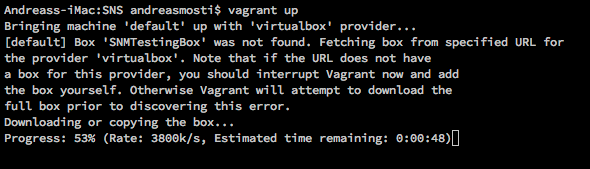
\includegraphics[scale = 0.7]{vagrantFirstTime.png}
\\ \\
Dette imaget er det vagrant kaller en ''box''. Den fungerer som grunnimage, og nedlastning skjer som sagt kun ved første gangs bygg av prosjektet. Ved alle nyoppsett av systemet vil imaget brukes som grunn-OS for prosjektfilene til SNS, eller en såkalt ''sandbox''. Boksen kan lokaliseres i den skjulte mappa ''./vagrant.d'' på hjemmekatalogen til brukeren din. \\ \\
For å sjekke at den virtuelle maskinen fungerer som den skal, gå til \url{http://localhost:8080/} fra nettleseren din. Du vil da få opp denne siden:
\\ \\
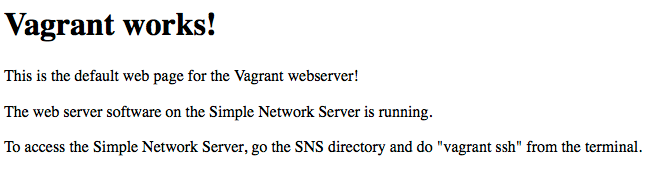
\includegraphics[scale = 0.7]{vagrantWorks.png} 
\\ \\

\subsection{Kjente oppsettsproblemer}
Den eneste feilen som har oppstått under testing er at versjonene av Virtualbox og Vagrant som ligger i repoene har vært ikke-kompatible med hverandre. Skulle dette oppstå ved oppsett, må man manuelt laste ned Virtualbox versjon 4.1.18 og legge denne inn. For 32 bit: 
\begin{lstlisting}
wget http://download.virtualbox.org/virtualbox/4.1.18/
virtualbox-4.1_4.1.18-78361~Ubuntu~precise_i386.deb
sudo dpkg -i virtualbox-4.1_4.1.18-78361~Ubuntu~precise_i386.deb
\end{lstlisting}
Og for 64 bit:
\\ 
\begin{lstlisting}
wget http://download.virtualbox.org/virtualbox/4.1.18/
virtualbox-4.1_4.1.18-78361~Ubuntu~precise_amd64.deb
sudo dpkg -i virtualbox-4.1_4.1.18-78361~Ubuntu~precise_amd64.deb
\end{lstlisting}
\\ 
Merk: Dette er pakker for Ubuntu 12.04 LTS. For andre versjoner av OS X / Linux, last ned fra \\
\url{https://www.virtualbox.org/wiki/Download_Old_Builds_4_1}
\\ \\ \\
Skulle problemer med Vagrant oppstå, kan også denne installeres utenom pakkesystemet. Da kjøres følgende (32 bit): 
\begin{lstlisting}
wget http://files.vagrantup.com/packages/7ec0ee1d00a916f80b109a298bab08e391945243/
vagrant_1.2.7_i686.deb 
sudo dpkg -i vagrant_1.2.7_i686.deb 
\end{lstlisting}
\\
Og for 64 bit - versjonen: 
\begin{lstlisting}
wget http://files.vagrantup.com/packages/7ec0ee1d00a916f80b109a298bab08e391945243/
vagrant_1.2.7_x86_64.deb
sudo dpkg -i vagrant_1.2.7_x86_64.deb
\end{lstlisting}
\\ 
Igjen, dette er pakker for Ubuntu. For andre distroer og OS X, besøk \\
\url{https://downloads.vagrantup.com/tags/v1.2.7} \\ \\
Erfaringer under testing har knyttet kjente problemer opp mot Virtualbox, så begynn med den.
\section{Arbeidsflyt}
Arbeidsflyten for produktet er veldig enkel. Når man står i prosjektets mappe, startes den virtuelle maskinen enkelt ved \\
\begin{lstlisting}
vagrant up
\end{lstlisting}
\\ 
Og maskinen aksesseres via SSH ved
\begin{lstlisting}
vagrant ssh
\end{lstlisting}
\\
Man blir da møtt av følgende skjermbilde: \\ \\
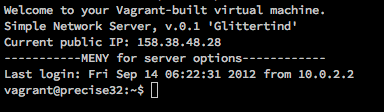
\includegraphics[scale = 0.7]{vagrantSSH.png}
\\ \\
og kan nå bruke alle verktøyene SNS tilbyr enkelt via kommandolinja, hovedsaklig via ''meny'' kommandoen for enkelhets skyld. Det er vert å merke seg at SNS - maskinen er en fullverdig virtuell Ubuntu - maskin, så all Linux - funksjonalitet utenfor prosjektets verktøy kan fritt brukes og / eller installeres. \\ 
Når man er ferdig med maskinen, avslutter man SSH - sesjonen og skriver: \\
\begin{lstlisting}
vagrant destroy
\end{lstlisting}
\\
Alle endringer og oppsett på den virtuelle maskinen blir nå slettet. Har man foreks. rotet det til med filer, angrepet serveren slik at den ikke lengre kan brukes fullstendig eller liknende, er ikke det noe problem. Nåværende system slettes. For neste gangs bruk av SNS, kjører man enkelt og greit ''vagrant up'' igjen, og prosjektet settes opp på nytt fra bunn av. 
\section{Gjennomgang av nåværende funksjonalitet}
For å benytte seg av funksjonaliteten som er bygget inn i SNS har vi laget en oppstartsmeny som enkelt og greit skal kunne guide deg til den funksjonaliteten du er ute etter (se kravdok). Du kommer til denne menyen når SNS er startet, og ''vagrant ssh'' er kjørt. Ved så å skrive ''meny'' fra kommandolinja, blir man møtt av følgende vindu: 
\\ \\
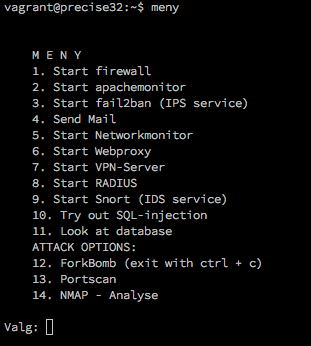
\includegraphics[scale=0.7]{meny.png} 
\\ \\
I dette avsnittet går vi gjennom hver av disse valgene, med forslag til bruk og utvidelse.  
\subsection{1: Start firewall}
Det første valget starter et skript som er tilpassed demonostrasjon av brannmur. \\ Her er funksjonaliteten ganske enkel: et skript starte brannmurprogrammvaren (ufw, abstraksjonslag oppå iptables) og laster inn en på forhånd oppsatt konfigurasjon som låser ned serveren, med unntak av portene som aktivt brukes i SNS som åpnes. Når skriptet er ferdig, dukker en oversikt over de åpne portene opp. 
\\ \\
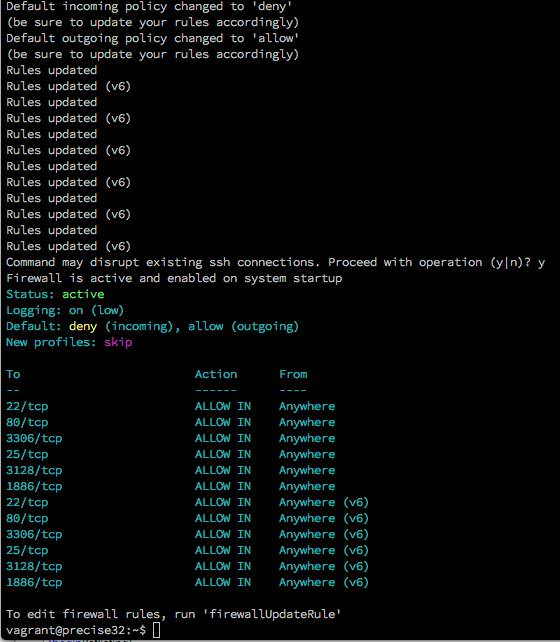
\includegraphics[scale = 0.7]{firewall.png}
\\ \\ 
Som vi ser av bildet, er de portene som er markert som åpne inn kun de som er ibruk av Simple Network Server. 
For å demonstrere brannmurendringern, kan skriptet 'firewallUpdateRule' kjøres rett fra kommandolinja. Dette skriptet er skrevet for enkelt og greit å gjøre endringer i aksesspolicyen til portene på serveren. Du velger om en port skal åpnes eller lukkes, og får da ny oversikt over portene på serveren. Dette for å lett kunne demonstrere brannmurens virkemåte. Eksemplel på bruk kan være å stenge port 80, for så å besøkle \url{http://localhost:8080} og se at aksessen nå er sperret. Anne bruk kan være å kjøre portscanner mot serverens adresse og se på åpne porter. 
\\ \\ 
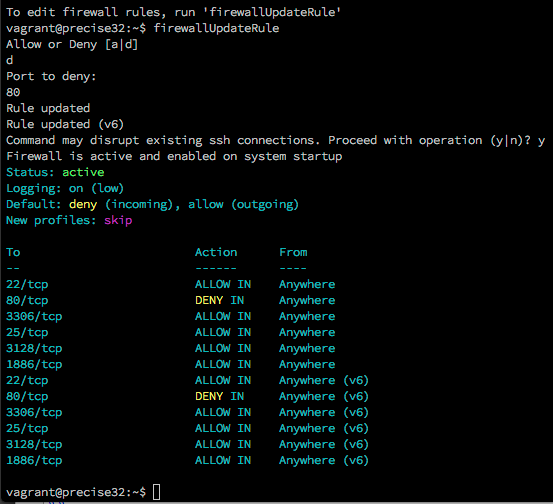
\includegraphics[scale =0.7]{firewallUpdate.png}
\\ \\
Eksempel på bruk av 'firewallUpdateRule', port 80 blir sperret.
\subsection{2: Start apachemonitor} 
Dette valget er ganske rett fram; et tilpasset skript deler skjermen i to og viser henholdsvis error og standard - loggen til webserveren apache2. Dette for å vise oppføringer som kommer når vi besøker sider hostet på webtjeneren, og kan vise hva som skjer når vi bestemmer oss for å ''plage'' LAMP - serveren.
\\ \\
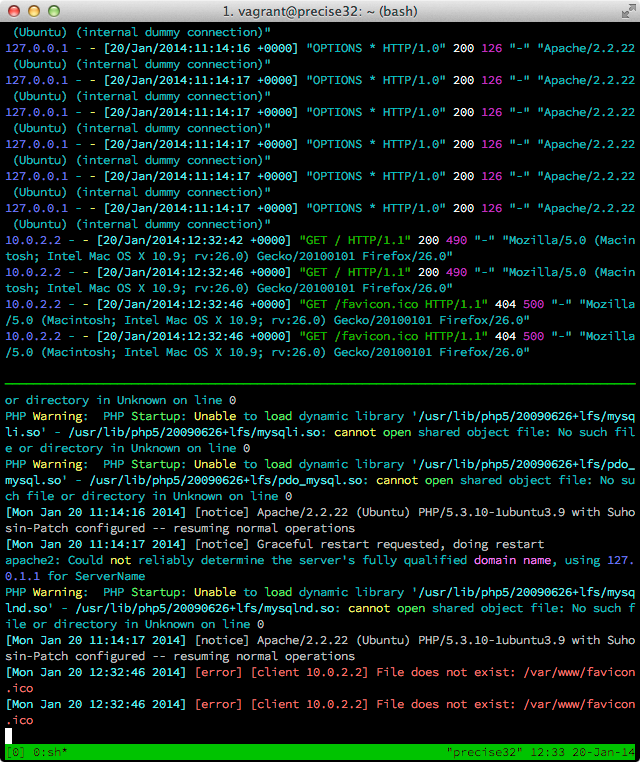
\includegraphics[scale= 0.7]{apachelogg.png}
\\ \\
Bildet viser eksempel på loggoppføring ved vanlig besøk på innhold hostet av webtjeneren. Leg merke til advarsel om fil som ikke eksisterer, denne feilen er framprovosert for å vise feil i loggen. Eksempel på bruk kan være å se hva som skjer i loggen om en modifisert get - request blir sendt. 
\subsection{3: Start fail2ban (IPS Service)}
En av de mest effektife Intrusion Prevention System - tjenestene der ute er fail2ban. Den banner rett og slett IP - adresser som prøver seg på bruteforce - angrep på serveren. Tjenesten starter rett og slett fail2ban etter en gitt tid. For å demonstrere bruk av fail2ban kan python-skriptet ''ssh\_forcer.py'' kjøres fra host - maskinen. Skriptet ligger på ''SNS/bin/Client/ssh\_forcer.py''. Skriptet trenger noen pakker for python, som kan skaffes ved å kjøre ''SNS/bin/pythonDependencies''. Skriptet vil prøve å brutforce SSH - login på SSN - serveren, passordforsøk på passordforsøk. Ved å aktivere fail2ban, kan man se at angrepsforsøkene stopper fordi IPen til slutt blir bannet. Effektiv demo av en IPS sine egenskaper: Den gjør aktive tiltak mot angriper.
\\ \\
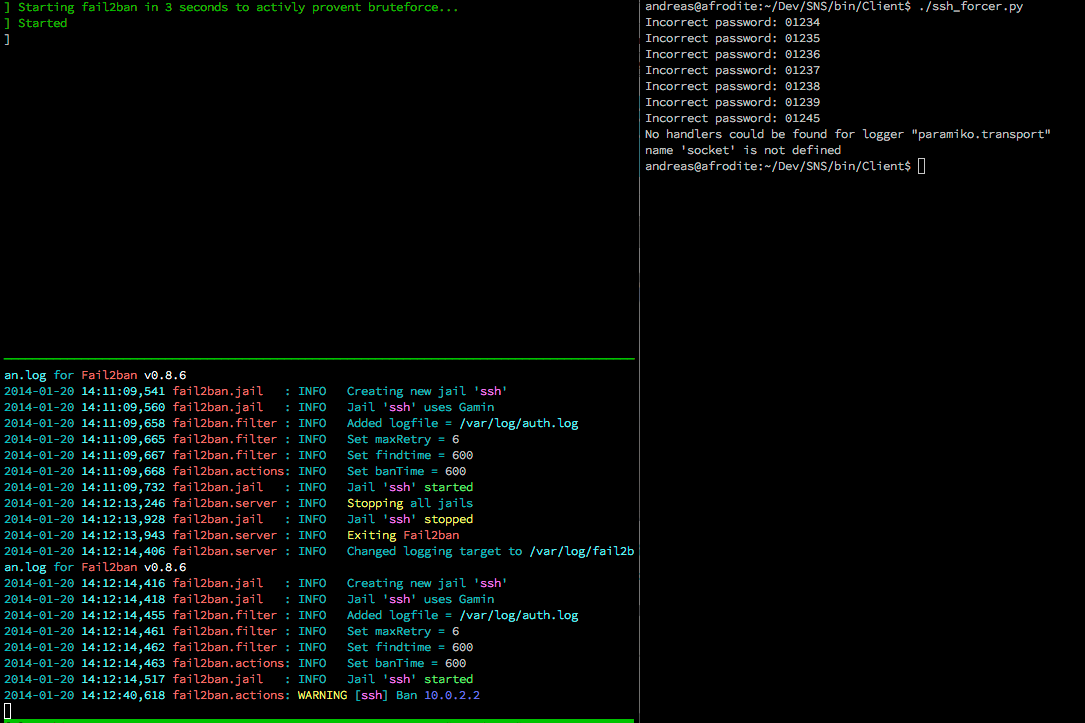
\includegraphics[scale = 0.5]{ips.png}
\\ \\
Bildet viser bruk av ssh\_forcer og IPS - pakken. Her får angriper prøvd seg 7 ganger før fail2ban starter og får sendt IPen i ''fengsel''. Utvidelse her kan være bruteforce - forsøk på HTTP - serveren. 
\subsection{4: Send mail}
Dette valget er ment som en demonstrasjon av hvor enkelt det er å sende epost med falsk avsender, som igjen kan føre til både pishingforsøk og spam. I dag regnes hele 80 - 85 \% av all mailtrafikk som spam.\footnote{Kilde: https://en.wikipedia.org/wiki/Spam_\%28electronic\%29#cite_note-4} Skriptet som starter mailsendingen spør deg om mottakeradresse (NB: ikke benytt skriptet uten at mottaker er klar over det!) og en ønsket avsenderadresses. Etter noen sekunder sendes mailen ut fra serveren, med en standard tekst som ligger lagret på ''/SNS/resources/doc/MailMessage''. \\ OBS: For at denne funksjonaliteten skal funke kan man \textit{ikke} være bak brannmur som stopper trafikk på SMTP - porten. Vanlige ISPer som Canal Digital osv. stopper trafikk her. Dette er derimot ikke et problem på HiST, hvor SNS hovedsaklig skal brukes. 
\\ \\
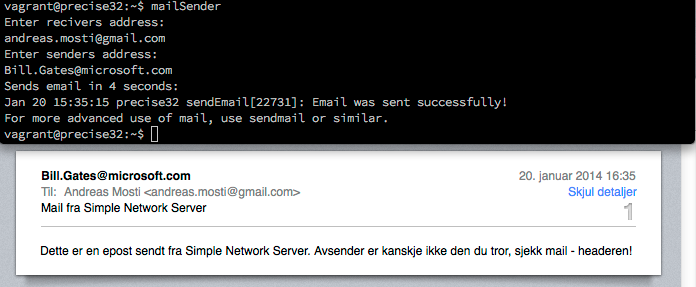
\includegraphics[scale = 0.7]{mailsender.png}
\\ \\ 
Her ser vi bruk av mailsender, hvor Bill Gates tilsynelatende har sendt mail. Men, som teksten sier, burde man sjekke mailheaderen for å se om avsender er den han er. Videre bruk av tjenesten kan være å lage til en phising - mal som sendes, for å demonstrere hvor enkelt det er å lage en tilsynelatende ekte mail fra foreks. banken din. Et annet bruksmønster er å overvåke pakkene som går; tjenesten er lagt opp til å sende mail uten kryptering, så alt går i klartekst. Dette er også grunnen til at mailen venter 4 sekunder før den sendes, så foreks. Wireshark kan rettes mot serverens IP for se på pakkene som går. 
\subsection{5: Start networkmonitor}
Dette valget er en nettverksmonitor satt sammen av programmene Nethogs og Iftop. Nethogs viser hvilke kjørende prosesser som genererer nettverkstrafikk, både innkommende og utgående, mens Iftop viser trafikk på eth0 - kortet, altså nettverkskortet på serveren. iftop viser hvilke IPer som blir kommunisert med, og hvor mye trafikk som går. Fordi SNS er bygget opp fra grun av med \textit{kun} den funksjonaliteten vi ønsker for å demonstrere forskjellige aspekter ved faget Nettverkssikkerhet, vil det være få prosesser som kjører (SNS er programmert til å blokkere alle tjenestene fra oppstart, de blir kun aktive når du velge å bruke dem) som igjen fører til en ren og ryddig logg: den blir ikke oversvømt av prosesser som bruker nettverk. Dette verktøyet er derfor veldig fint å bruke for å demonstrere hvordan prosesser bruker trafikk inn / ut av serveren. 
\\ \\
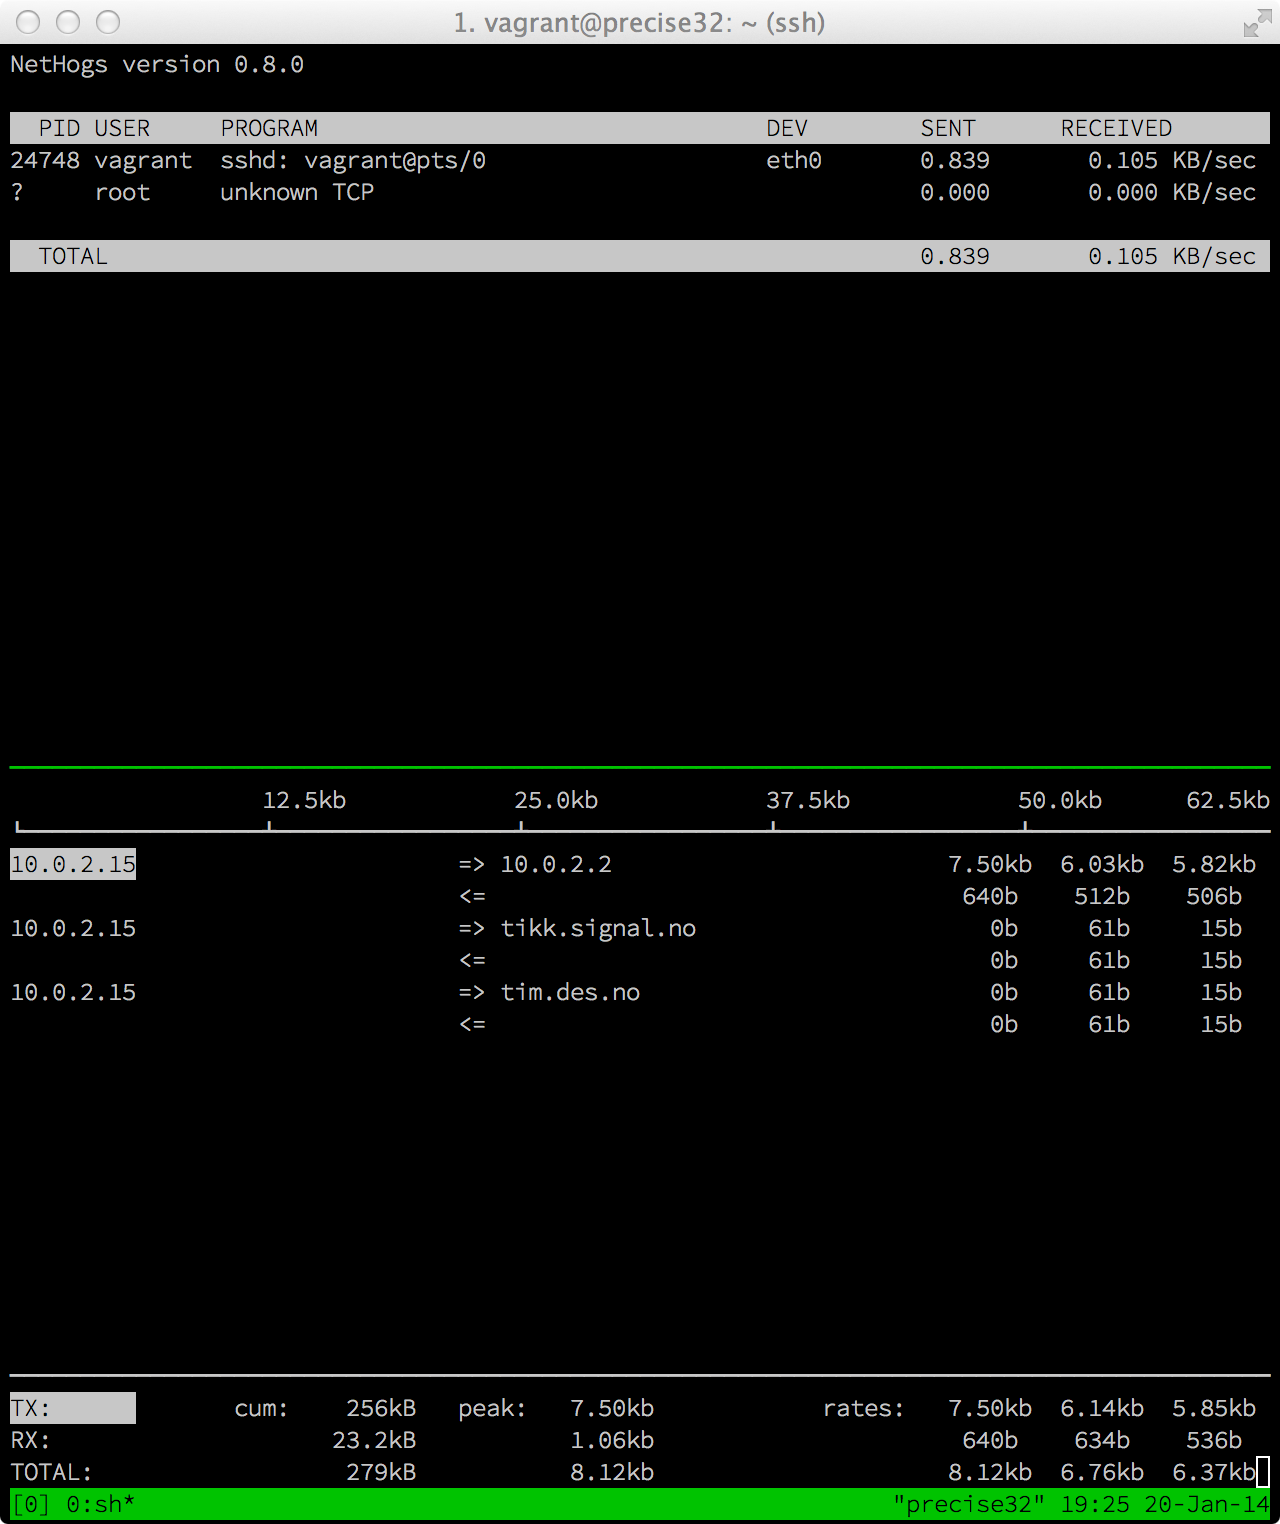
\includegraphics[scale = 0.6]{networkmonitor.png} 
\\ \\
Det øverste vinduet er Nethogs, som her kun viser en aktiv prosess som bruker av nettverket, nemmlig SSH, som jeg kommuniserer med serveren via. \\ 
Nedenfor ser vi iftop som melder om trafikk fra serveren til 10.0.2.2 som er hostmaskinens IP, samt trafikk til Signal, som er ISP der serveren står.
Forslag bruk av denne netverksmonitoren er som nevnt å vise hvordan trafikk til / fra serveren vises, og man kan demonstrere hvor greit det er å holde orden på hvilke prosesser som bruker nettverksresurser i systemet. Skulle serveren bli kompromitert og bli en del av et botnet, kan man da helt klart se av monitoren om noe genererer mye trafikk. 
\section{Om kildekodens oppbyggning}
<her kommer beskrivelse av mappestruktur>

\end{document}